\documentclass[a4paper, oneside, 12pt]{article}
\usepackage[english, romanian]{babel}
\usepackage[utf8]{inputenc}
\usepackage{pdfpages}
\usepackage{indentfirst}
\usepackage{listings}
\usepackage{xcolor}
\usepackage[margin=0.5in]{geometry}
\usepackage{textcomp}
\usepackage{mathptmx}
\usepackage{color}
\usepackage{pdflscape}
\usepackage[hidelinks]{hyperref}
\usepackage{enumitem}
\usepackage[T1]{fontenc}
\usepackage[scaled=0.9]{DejaVuSansMono}
\usepackage[stable]{footmisc}
\usepackage{xspace}
\usepackage{caption}
\usepackage{float}
\usepackage{import}
\usepackage{xifthen}
\usepackage{transparent}

\definecolor{codegreen}{rgb}{0,0.6,0}
\definecolor{codegray}{rgb}{0.5,0.5,0.5}
\definecolor{codepurple}{HTML}{C42043}
\definecolor{backcolour}{HTML}{F2F2F2}
\definecolor{bookColor}{cmyk}{0,0,0,0.90}  
\color{bookColor}

\lstset{upquote=true}

\lstdefinestyle{sqlstyle}{
    backgroundcolor=\color{backcolour},   
    commentstyle=\color{gray},
    keywordstyle=\color{codepurple},
    numberstyle=\numberstyle,
    stringstyle=\color{codepurple},
    basicstyle=\footnotesize\ttfamily,
    breakatwhitespace=false,
    breaklines=true,
    captionpos=b,
    keepspaces=true,
    numbers=left,
    numbersep=10pt,
    showspaces=false,
    showstringspaces=false,
    showtabs=false,
    language=SQL,
    deletekeywords={IDENTITY},
    deletekeywords={[2]INT},
    morekeywords={clustered},
    framesep=8pt,
    xleftmargin=40pt,
    framexleftmargin=40pt,
    frame=tb,
    framerule=0pt
}
\lstset{style=sqlstyle}

\newcommand\numberstyle[1]{%
    \footnotesize
    \color{codegray}%
    \ttfamily
    \ifnum#1<10 0\fi#1 |%
}

\newlist{m_itemize}{itemize}{1}
\setlist[m_itemize]{label=\textbullet, noitemsep, topsep=0pt, after=\vspace{.4\baselineskip}}

\newcommand{\str}{variabilă de tip \emph{șir de caractere}\xspace}
\newcommand{\nump}{variabilă de tip \emph{număr natural de maxim 3 cifre}\xspace}
\newcommand{\numpp}{variabilă de tip \emph{număr natural de maxim 5 cifre}\xspace}
\newcommand{\datet}{variabilă de tip \emph{dată calendaristică}\xspace}
\newcommand{\nnull}{variabilă de tip \emph{not null}\xspace}

\usepackage{array}
\newcolumntype{$}{>{\global\let\currentrowstyle\relax}}
\newcolumntype{^}{>{\currentrowstyle}}
\newcommand{\rowstyle}[1]{\gdef\currentrowstyle{#1}%
  #1\ignorespaces
}

\newcommand{\incfig}[1]{%
    \def\svgwidth{\columnwidth}
    \import{./../../img/}{#1.pdf_tex}
}

\title{Management-ul unui magazin de muzică}
\author{Nicula Ionuț-Cosmin \\ \emph{mail: }\texttt{ionut.nicula@s.unibuc.ro} \\\hspace{35pt}\texttt{niculaionut@tutanota.com}
\\ \emph{surse: }\texttt{github.com/niculaionut/proiect-bd}}

\begin{document}

\maketitle

\newpage

\tableofcontents

\newpage

\section{Descrierea modelului și a utilității acestuia}

\section{Constrângerile impuse asupra modelului}

\section{Descrierea entităților}

Numele entităților, împreună cu descrierea acestora:

\begin{enumerate}[noitemsep, label=\roman*.]

\item \textbf{COUNTRY}:
        \begin{m_itemize}
                \item Entitate care identifică țara unei anumite locații.
        \end{m_itemize}

\item \textbf{LOCATION}:
        \begin{m_itemize}
                \item Entitate care identifică locația în care s-a născut un anumit artist.
        \end{m_itemize}

\item \textbf{ARTIST}:
        \begin{m_itemize}
                \item Persoană care participă la compunerea unor creații muzicale.
        \end{m_itemize}

\item \textbf{GROUP}:
        \begin{m_itemize}
                \item Entitate care reprezintă o mulțime de unul sau mai mulți artiști.
        \end{m_itemize}

\item \textbf{ALBUM}:
        \begin{m_itemize}
                \item Entitate care reprezintă o colecție de compoziții muzicale.
        \end{m_itemize}

\item \textbf{TRACK}:
        \begin{m_itemize}
                \item Entitate care reprezintă un track individual din componența unui album.
        \end{m_itemize}

\item \textbf{CATEGORY}:
        \begin{m_itemize}
                \item Entitate ce identifică din ce categorie muzicală face parte un album.
        \end{m_itemize}

\item \textbf{COPY}:
        \begin{m_itemize}
                \item Entitate care reprezintă o copie fizică a unui album.
        \end{m_itemize}

\item \textbf{CUSTOMER}:
        \begin{m_itemize}
                \item Entitate care reprezintă un client înregistrat pe site-ul magazinului.
                \item Acesta poate cumpăra copii fizice ale albumelor și se
                      poate abona la categoriile disponibile pe site-ul magazinului.
        \end{m_itemize}

\item \textbf{EMPLOYEE}:
        \begin{m_itemize}
                \item Entitate care reprezintă un angajat al magazinului.
                \item În funcție de job, anagajatul desfășoară anumite activități.
        \end{m_itemize}

\item \textbf{JOB}:
        \begin{m_itemize}
        \item Entitate care identifică job-ul unui angajat (ex: îngrijitor, manager, asociat vânzări, etc.).
        \end{m_itemize}

\end{enumerate}

Entitatea \textbf{Track} are drept cheie primară perechea \textbf{<album\_id, id>}.

Entitatea \textbf{Copy} are drept cheie primară perechea \textbf{<album\_id, id>}.

Fiecare entitate dintre toate celelalte are în componență un atribut \textbf{id} care reprezintă cheia primară.


\section{Descrierea relațiilor}
\label{descrel}

\begin{enumerate}[noitemsep, label=\roman*.]

\item \textbf{LOCATION} \emph{se află în} \textbf{COUNTRY}:
        \begin{m_itemize}%[noitemsep, topsep=0pt, after=\vspace{.5\baselineskip}]
                \item Identifică țara în care se află o locație.
                \item Are cardinalitatea {\texttt{M(0):1(1)}.}
        \end{m_itemize}

\item \textbf{ARTIST} \emph{este născut în} \textbf{LOCATION}:
        \begin{m_itemize}
                \item Identifică locația în care un artist este născut.
                \item Are cardinalitatea {\texttt{M(0):1(1)}.}
        \end{m_itemize}

\item \textbf{ARTIST} \emph{face parte din} \textbf{GROUP}:
        \begin{m_itemize}
                \item Realizează legătura dintre artist și grupurile din care face parte.
                \item Are cardinalitatea {\texttt{M(1):M(0)}.}
        \end{m_itemize}

\item \textbf{ALBUM} \emph{este compus de} \textbf{GROUP}:
        \begin{m_itemize}
                \item Realizează legătura dintre album și grupul de care este compus.
                \item Are cardinalitatea {\texttt{M(0):1(1)}.}
        \end{m_itemize}

\item \textbf{TRACK} \emph{face parte din} \textbf{ALBUM}:
        \begin{m_itemize}
                \item Face legătura dintre album și track-urile din componența sa.
                \item Are cardinalitatea {\texttt{M(1):1(1)}.}
        \end{m_itemize}

\item \textbf{ALBUM} \emph{face parte din} \textbf{CATEGORY}:
        \begin{m_itemize}
                \item Realizează legătura dintre album și categoria din care acesta face parte.
                \item Are cardinalitatea {\texttt{M(0):1(1)}.}
        \end{m_itemize}

\item \textbf{COPY} \emph{este copie a albumului} \textbf{ALBUM}:
        \begin{m_itemize}
                \item Realizează legătura dintre album și copiile fizice ale acestuia.
                \item Are cardinalitatea {\texttt{M(0):1(1)}.}
        \end{m_itemize}

\item \textbf{EMPLOYEE} \emph{este angajat ca} \textbf{JOB}:
        \begin{m_itemize}
                \item Realizează legătura dintre angajat și job-ul său.
                \item Are cardinalitatea {\texttt{M(0):1(1)}.}
        \end{m_itemize}

\item \textbf{CUSTOMER} \emph{cumpără} \textbf{COPY}:
        \begin{m_itemize}
                \item Realizează legătura dintre client și copiile pe care acesta le-a cumpărat.
                \item Are cardinalitatea {\texttt{1(0):M(0)}.}
        \end{m_itemize}

\item \textbf{CUSTOMER} \emph{se abonează la} \textbf{CATEGORY} \emph{prin intermediul} \textbf{EMPLOYEE}:
        \begin{m_itemize}
                \item Realizează legătura dintre client, categorie și angajat;
                \item Reprezintă un abonament prin prisma căruia se pot trimite clientului oferte, reduceri, etc;
                \item Are cardinalitatea \texttt{M(0):M(0):M(0)}.
        \end{m_itemize}

\end{enumerate}

\section{Descrierea atributelor}

Numele entităților, împreună cu numele atributelor și descrierea fiecăruia:

\begin{enumerate}[noitemsep, label=\roman*.]

\item \textbf{COUNTRY}:
        \begin{m_itemize}
                \item \emph{id}: \nump care reprezintă id-ul țării;
                \item \emph{name}: \str\footnote{Toate atributele de tip
                      \emph{șir de caractere} vor avea lungimea maximă egală
                      cu 50.} care reprezintă numele țării.
        \end{m_itemize}

\item \textbf{LOCATION}:
        \begin{m_itemize}
                \item \emph{id}: \nump  care reprezintă id-ul locației;
                \item \emph{city}: \str care reprezintă numele orașului locației.
        \end{m_itemize}

\item \textbf{ARTIST}:
        \begin{m_itemize}
                \item \emph{id}: \nump care reprezintă id-ul artistului;
                \item \emph{first\_name}: \str care reprezintă prenumele artistului;
                \item \emph{last\_name}: \str care reprezintă numele artistului;
                \item \emph{date\_birth}: \datet care reprezintă data nașterii artistului;
                \item \emph{date\_birth}: \datet care reprezintă data decesului artistului.
        \end{m_itemize}

\item \textbf{GROUP}:
        \begin{m_itemize}
                \item \emph{id}: \nump care reprezintă id-ul grupului;
                \item \emph{name}: \str care reprezintă numele grupului.
        \end{m_itemize}

\item \textbf{ALBUM}:
        \begin{m_itemize}
                \item \emph{id}: \nump care reprezintă id-ul albumului;
                \item \emph{title}: \str care reprezintă numele albumului;
                \item \emph{release\_date}: \datet care reprezintă data la care s-a lansat albumul.
        \end{m_itemize}

\item \textbf{TRACK}:
        \begin{m_itemize}
                \item \emph{album\_id}: \nump care reprezintă id-ul albumului din care face parte track-ul;
                \item \emph{id}: \nump care reprezintă id-ul track-ului;
                \item \emph{title}: \str care reprezintă titlul track-ului;
                \item \emph{length}: \numpp care reprezintă durata în minute a track-ului.
        \end{m_itemize}

\item \textbf{CATEGORY}:
        \begin{m_itemize}
                \item \emph{id}: \nump care reprezintă id-ul categoriei;
                \item \emph{title}: \str care reprezintă titlul categoriei.
        \end{m_itemize}

\item \textbf{COPY}:
        \begin{m_itemize}
                \item \emph{album\_id}: \nump care reprezintă id-ul albumului copiei fizice;
                \item \emph{id}: \nump care reprezintă id-ul copiei;
                \item \emph{serial\_number}: \str care reprezintă numărul de serie (unic) al copiei;
                \item \emph{price}: \numpp care reprezintă prețul copiei.
        \end{m_itemize}

\item \textbf{CUSTOMER}:
        \begin{m_itemize}
                \item \emph{id}: \nump care reprezintă id-ul clientului;
                \item \emph{first\_name}: \str care reprezintă prenumele clientului;
                \item \emph{last\_name}: \str care reprezintă numele clientului;
                \item \emph{email}: \str care reprezintă email-ul clientului.
        \end{m_itemize}

\item \textbf{EMPLOYEE}:
        \begin{m_itemize}
                \item \emph{id}: \nump care reprezintă id-ul angajatului;
                \item \emph{first\_name}: \str care reprezintă prenumele angajatului;
                \item \emph{last\_name}: \str care reprezintă numele angajatului;
                \item \emph{salary}: \numpp care reprezintă salariul angajatului;
                \item \emph{hire\_date}: \datet care reprezintă data angajării angajatului.
        \end{m_itemize}

\item \textbf{JOB}:
        \begin{m_itemize}
                \item \emph{id}: \nump care reprezintă id-ul job-ului;
                \item \emph{title}: \str care reprezintă titlul job-ului;
                \item \emph{min\_salary}: \numpp care reprezintă salariul minim al job-ului;
                \item \emph{max\_salary}: \numpp care reprezintă salariul maxim job-ului.
        \end{m_itemize}

\end{enumerate}

\section{Diagrama entitate-relație\footnote{pe pagina următoare}}

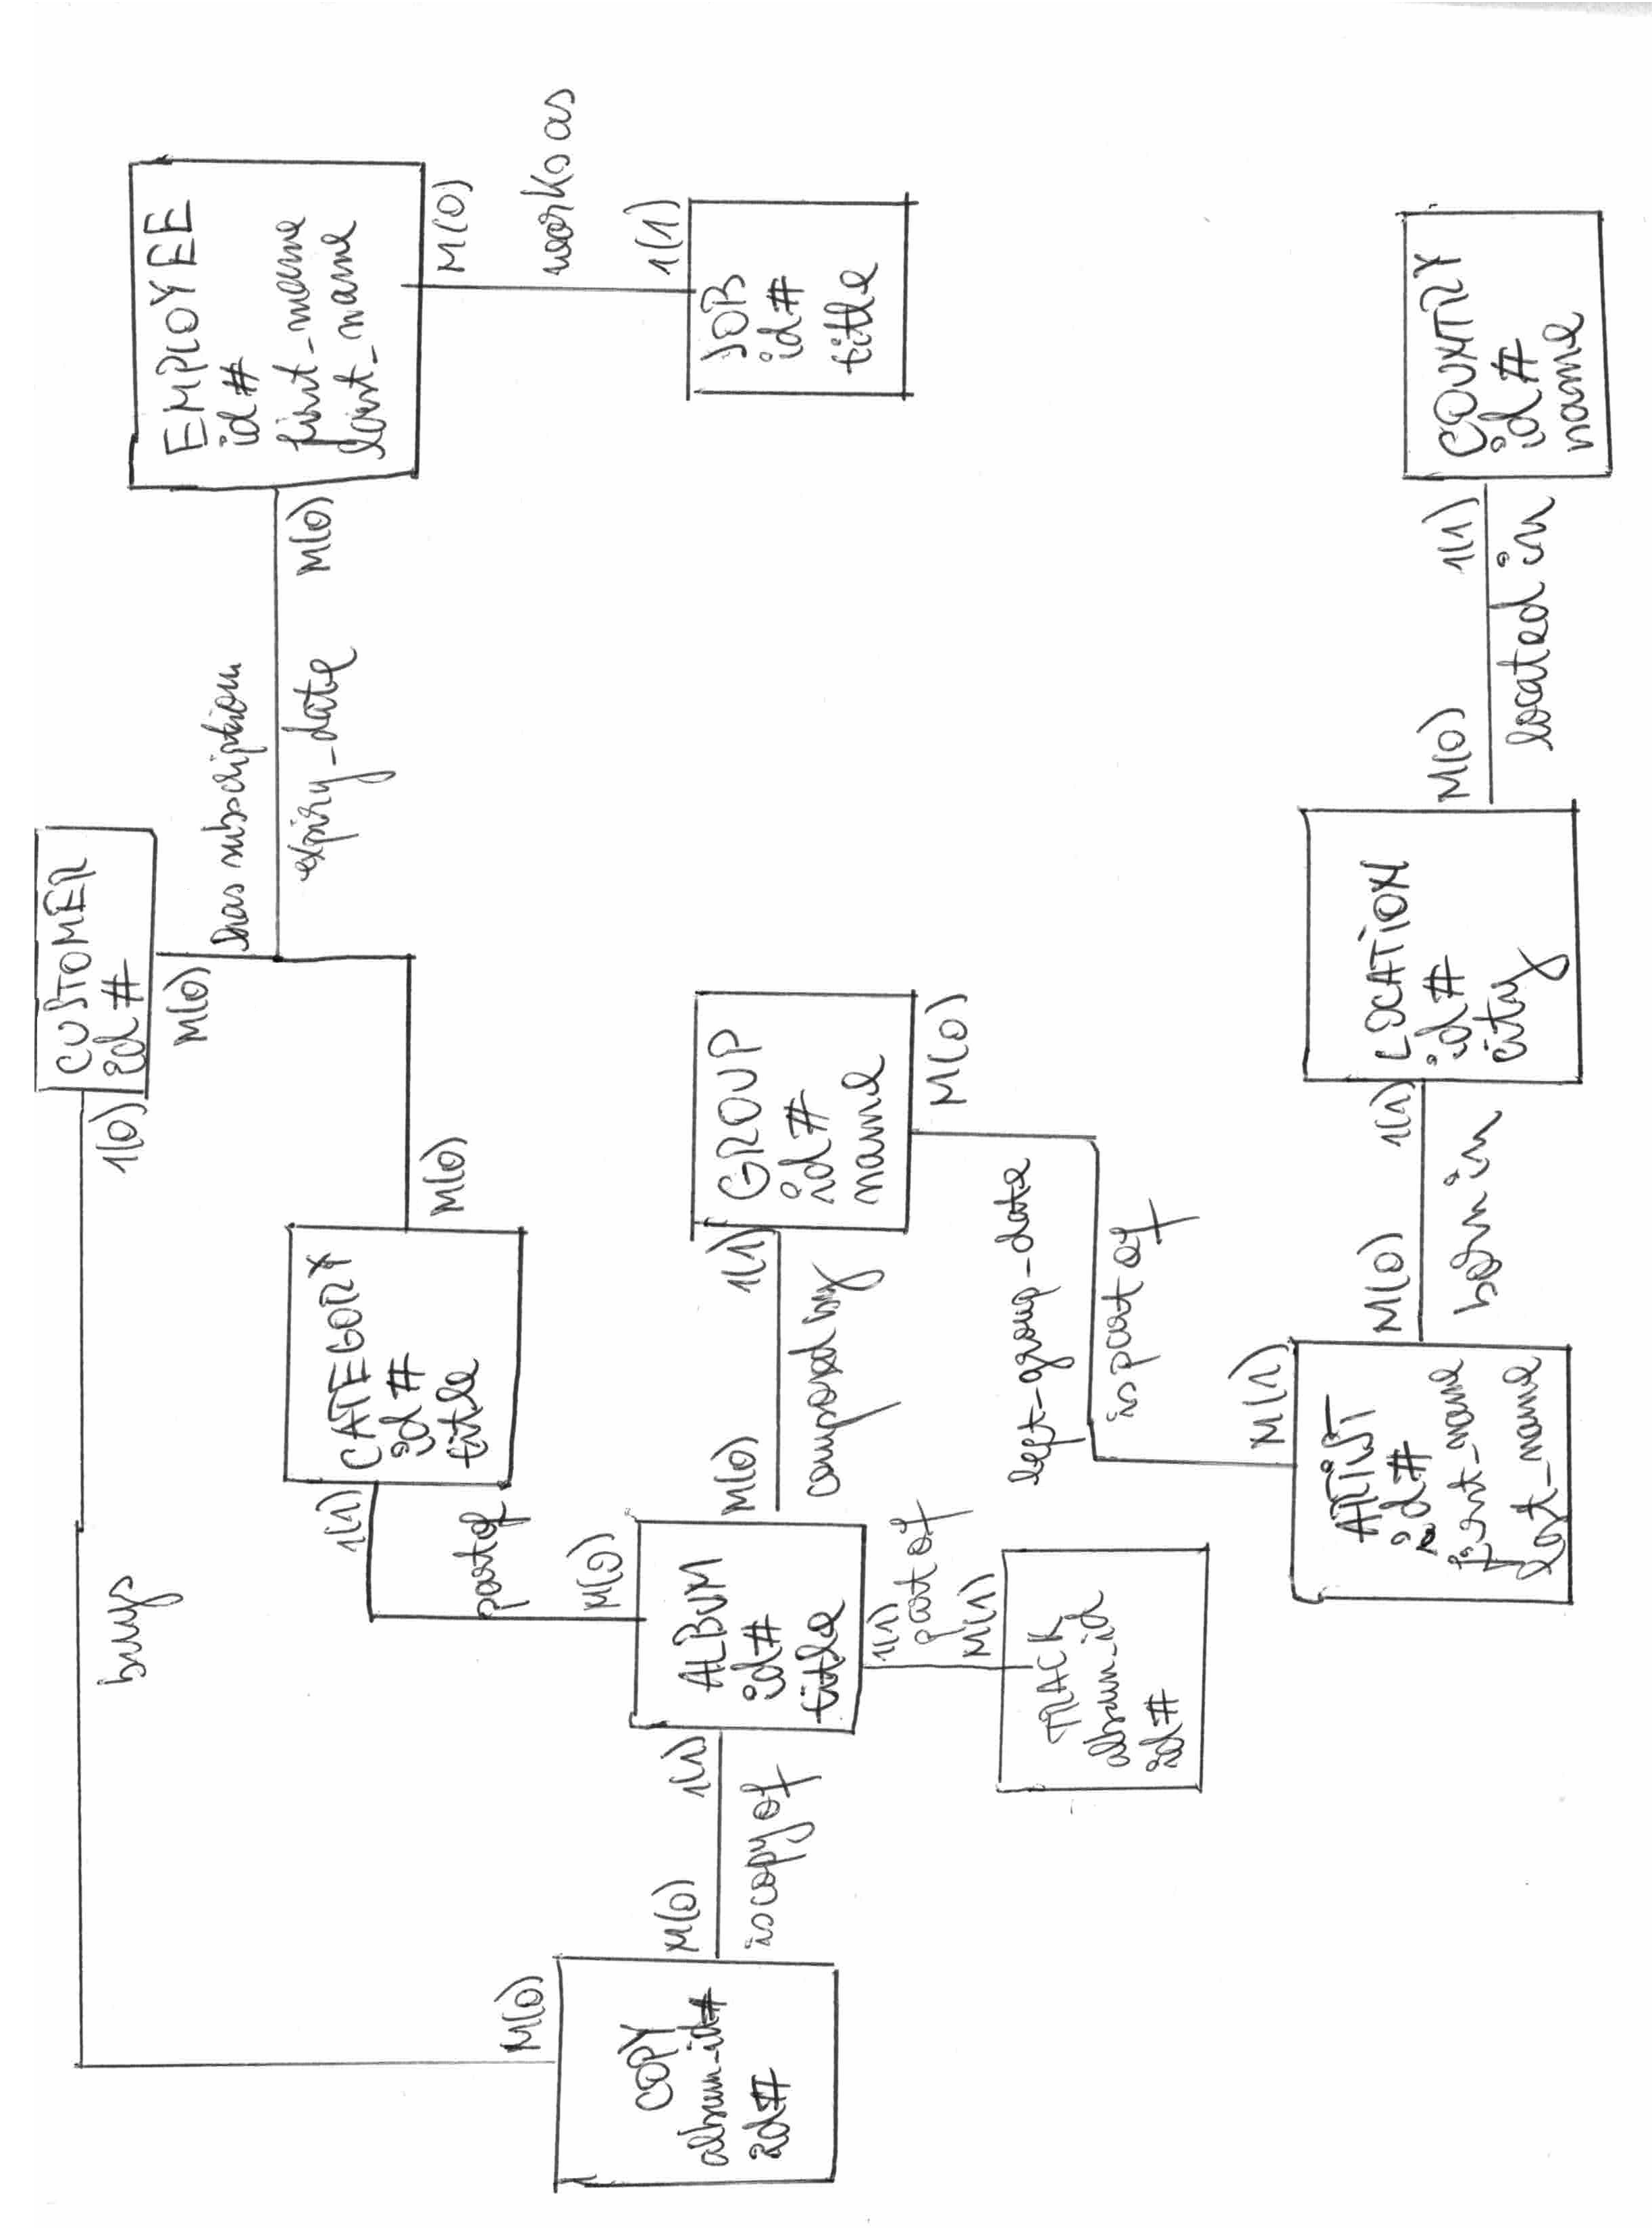
\includepdf[pages=-]{../../img/diagrama_er.png}

\section{Diagrama conceptuală\footnote{pe pagina următoare}}

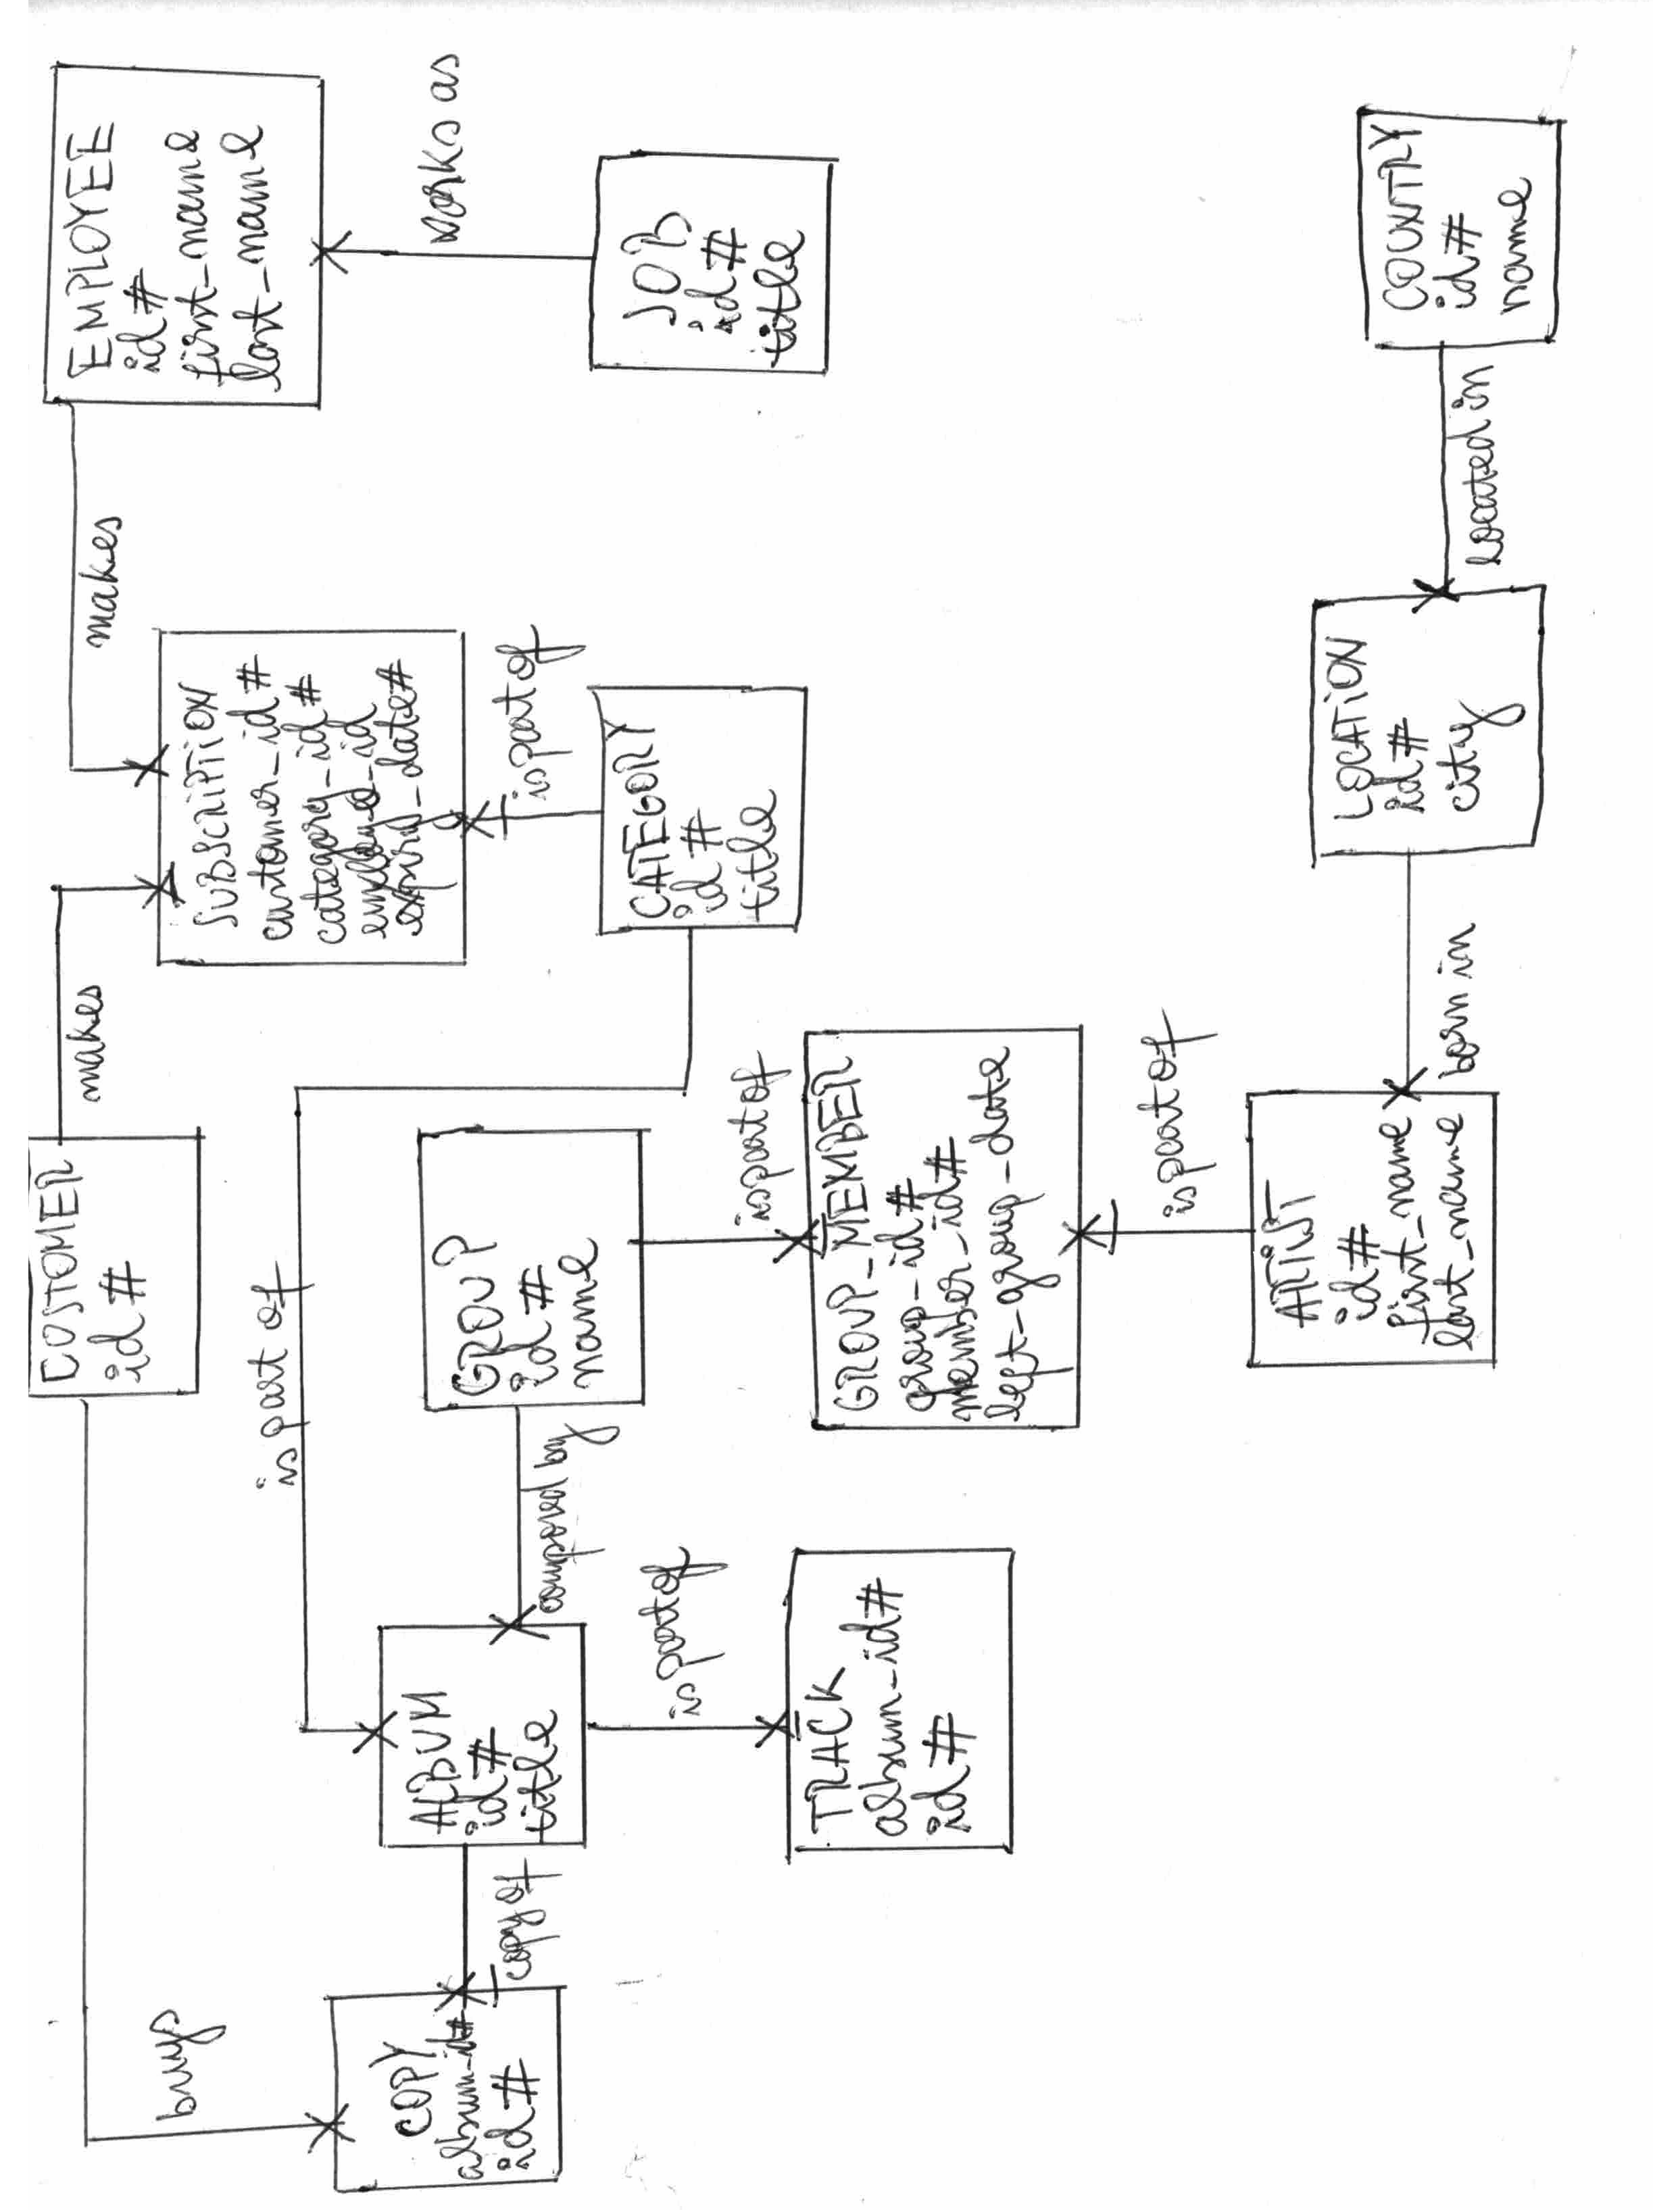
\includepdf[pages=-]{../../img/diagrama_conceptuala.png}

\section{Schemele relaționale}

\begin{center}

\lstinputlisting[language=C]{../../generate/schema_relationala.txt}

\end{center}

\section{Normalizarea până la forma normală 3}

\subsection{FN1}

Se ia ca exemplu de \textbf{non-FN1} tabela \textbf{ALBUMS\_0}, având următoarele atribute și înregistrări:

% inainte de normalizare

\begin{table}[h]
\centering
\caption*{Tabela \textbf{ALBUMS\_0}:}
\begin{tabular}{$c^c^c^c}
        \hline
        \rowstyle{\bfseries}
        id\# & group\_id & title & tracks \\
        \hline
        1 & 1 & Animals & Pigs, Dogs, Sheep \\
        \hline
        2 & 2 & Goldberg Variations (Excerpts) & Aria, Variation 1, Variation 2, Variation 16\\
        \hline
\end{tabular}
\end{table}

Deoarece \textbf{FN1} nu admite atribute cu valori non-atomice,
\textbf{ALBUMS\_0} se împarte în două tabele.

\textbf{ALBUMS\_1} conține
toate atributele din \textbf{ALBUMS\_0} cu excepția celui cu valori multiple,
iar \textbf{ALBUMS\_2} conține câte o înregistrare separată pentru fiecare
track asociat albumului.

Printr-o operație de \emph{join} între cele două tabele obținute, se accesează
(fără pierdere de informație) toate track-urile din componența unui album.

% dupa normalizare


\begin{table}[h]
\centering
\caption*{Tabela \textbf{ALBUMS\_1}:}
\begin{tabular}{$c^c^c}
        \hline
        \rowstyle{\bfseries}
        id\# & group\_id & title \\
        \hline
        1 & 1 & Animals \\
        \hline
        2 & 2 & Goldberg Variations (Excerpts) \\
        \hline
\end{tabular}
\end{table}

\begin{table}[H]
\centering
\caption*{Tabela \textbf{ALBUMS\_2}:}
\begin{tabular}{$c^c}
        \hline
        \rowstyle{\bfseries}
        id\# & track \\
        \hline
        1 & Pigs \\
        \hline
        1 & Dogs \\
        \hline
        1 & Sheep \\
        \hline
        2 & Aria \\
        \hline
        2 & Variation 1 \\
        \hline
        2 & Variation 2 \\
        \hline
        2 & Variation 16 \\
        \hline
\end{tabular}
\end{table}

\subsection{FN2}

Se ia ca exemplu de \textbf{non-FN2} tabela \textbf{GROUP\_MEMBER\_0} care face
legătura dintre grupuri și membrii componenți ai acestora. Un grup poate avea
mai mulți membri iar un artist poate face parte din mai multe grupuri.

% inainte de normalizare

\begin{table}[H]
\centering
\caption*{Tabela \textbf{GROUP\_MEMBER\_0}:}
\begin{tabular}{$c^c^c^c}
        \hline
        \rowstyle{\bfseries}
        group\_id\# & member\_id\# & left\_group\_date & first\_name \\
        \hline
        1 & 1 & null & Nick \\
        \hline
        1 & 2 & null & David \\
        \hline
\end{tabular}
\end{table}

Deoarece valorile \textbf{first\_name} depind doar de al doilea component
(\textbf{member\_id\#}) al cheii primare, tabela inițială se împarte în două alte tabele,
cu scopul eliminării dependenței parțiale; tabelele rezultate respectă proprietățile \textbf{FN2}.

\begin{table}[H]
\centering
\caption*{Tabela \textbf{GROUP\_MEMBER\_1}:}
\begin{tabular}{$c^c^c}
        \hline
        \rowstyle{\bfseries}
        group\_id\# & member\_id\# & left\_group\_date \\
        \hline
        1 & 1 & null \\
        \hline
        1 & 2 & null \\
        \hline
\end{tabular}
\end{table}

\begin{table}[H]
\centering
\caption*{Tabela \textbf{GROUP\_MEMBER\_2}:}
\begin{tabular}{$c^c}
        \hline
        \rowstyle{\bfseries}
        member\_id\# & first\_name \\
        \hline
        1 & Nick \\
        \hline
        2 & David \\
        \hline
\end{tabular}
\end{table}

\subsection{FN3}

Se ia ca exemplu de \textbf{non-FN3} tabela \textbf{SUBSCRIPTION\_0} care
realizează legătura dintre un client, categoria la care este sau a fost
abonat\footnote{Pe parcursul rezolvării cerințelor se folosește și formularea
\emph{„client \textbf{este} abonat la categorie”}. Acolo unde nu se precizează dacă
abonamentul este activ sau expirat, a se înțelege sensul formulării tot drept \emph{„client este
\textbf{sau a fost} abonat la categorie”}.}, și angajatul prin intermediul
căruia s-a realizat abonamentul. O înregistrare de tip abonament aparține unui
singur client. Un client poate avea mai multe abonamente asociate; o categorie
poate avea mai multe abonamente asociate; un angajat poate crea mai multe
abonamente.


\begin{table}[H]
\centering
\caption*{Tabela \textbf{SUBSCRIPTION\_0}:}
\begin{tabular}{$c^c^c^c^c}
        \hline
        \rowstyle{\bfseries}
        customer\_id\# & category\_id\# & employee\_id & expiry\_date\# & employee\_first\_name \\
        \hline
        1 & 10 & 5 & 19/03/2020 & Tracy\\
        \hline
        2 & 10 & 3 & 02/01/2019 & John\\
        \hline
\end{tabular}
\end{table}

Se observă că atributele care nu participă la cheia primară sunt dependente de
\emph{întregimea} cheii primare, deci structura respectă proprietățile \textbf{FN2}.
Totuși, atributul \textbf{employee\_first\_name} este dependent în mod
\emph{tranzitiv} de cheia primară.

Pentru a elimina dependența tranzitivă, tabela se împarte în următoarele două
componente al căror \emph{join} păstrează accesul la aceleași informații din
tabela inițială:

\begin{table}[H]
\centering
\caption*{Tabela \textbf{SUBSCRIPTION\_1}:}
\begin{tabular}{$c^c^c^c^c}
        \hline
        \rowstyle{\bfseries}
        customer\_id\# & category\_id\# & employee\_id & expiry\_date\# \\
        \hline
        1 & 10 & 5 & 19/03/2020 \\
        \hline
        2 & 10 & 3 & 02/01/2019 \\
        \hline
\end{tabular}
\end{table}

\begin{table}[H]
\centering
\caption*{Tabela \textbf{SUBSCRIPTION\_2}:}
\begin{tabular}{$c^c}
        \hline
        \rowstyle{\bfseries}
        employee\_id\# & employee\_first\_name \\
        \hline
        5 & Tracy \\
        \hline
        3 & John \\
        \hline
\end{tabular}
\end{table}

\section{Crearea tabelelor și inserarea de date coerente}

screenshots go here

\section{Cinci cereri SQL complexe}

\begin{center}

\minipage{\linewidth}
\lstinputlisting[caption=\centering{Operație \emph{join} pe minimum 4 tabele{,}
filtrare la nivel de linii{,} subcerere nesincronizată{,} ordonare{,} funcții
pe șiruri de caractere}]{../../queries/1.sql}
\endminipage

\minipage{\linewidth}
\lstinputlisting[caption=\centering{Subcerere sincronizată{,} grupări{,}
funcții grup{,} filtrare la nivel de grupuri{,} operații pe șiruri de
caractere}]{../../queries/2.sql}
\endminipage

\minipage{\linewidth}
\lstinputlisting[caption=\texttt{NVL}{,} \texttt{DECODE}{,} \texttt{CASE}{,}
funcții pe date calendaristice{,} funcții pe șiruri de
caractere]{../../queries/3.sql}
\endminipage

\minipage{\linewidth}
\lstinputlisting[caption=Clauza \texttt{WITH}]{../../queries/4.sql}
\endminipage

\minipage{\linewidth}
\lstinputlisting[caption=Funcții pe date calendaristice]{../../queries/5.sql}
\endminipage

\end{center}

\section{Operații de actualizare/suprimare utilizând subcereri}

\begin{center}

\minipage{\linewidth}
\lstinputlisting[caption=Suprimare/Actualizare utilizând subcereri]{../../queries/6.sql}
\endminipage

\end{center}

\section{Crearea unei secvențe utilizate în inserarea unor înregistrari în tabele}

Secvența următoare este folosită la introducerea datelor în tabela
\texttt{Artists}. Generează un ID unic pentru fiecare înregistrare.

\begin{center}

\minipage{\linewidth}
\lstinputlisting[caption=Crearea secvenței]{../../generate/create-sequence.sql}
\endminipage

\minipage{\linewidth}
\lstinputlisting[caption=Exemplu de inserare folosind secvența]{../../generate/sequence-example.sql}
\endminipage

\end{center}

\section{Cereri cu operații \emph{outer-join} și \emph{division}}

\begin{center}

\minipage{\linewidth}
\lstinputlisting[caption=Cerere cu operație \emph{outer-join}]{../../queries/21.sql}
\endminipage

\end{center}

\section{Realizarea normalizării la formele superioare, aplicarea denormalizării}

\subsection{Normalizarea la \textbf{BCNF}, \textbf{FN4}, \textbf{FN5}}

\subsubsection{\textbf{BCNF}}

Se consideră ca exemplu \textbf{non-BCNF} relația:

\begin{m_itemize}
        \item \textbf{FREQUENT\_0 (category\_id\#, customer\_email\#, customer\_id)}
\end{m_itemize}

Relația face legătura dintre un client și categoriile pe care le frecventează des (pe site-ul magazinului).
O categorie poate fi frecventată de mai mulți clienți, iar un client poate
frecventa mai multe categorii. Clienții au email-uri și id-uri unice.

Astfel, se observă dependențele funcționale:

\begin{m_itemize}
        \item \{category\_id\#, customer\_email\#\} $\rightarrow$ \{customer\_id\};
        \item \{customer\_id\} $\rightarrow$ \{customer\_email\#\}.
\end{m_itemize}

Deoarece \textbf{customer\_id} nu este o cheie candidat, relația trebuie
împărțită în următoarele două componente pentru a respecta proprietățile
\textbf{BCNF}:

\begin{m_itemize}
        \item \textbf{FREQUENT\_1 (customer\_id\#, customer\_email)}
        \item \textbf{FREQUENT\_2 (category\_id\#, customer\_id\#)}
\end{m_itemize}

\subsubsection{\textbf{FN4}}

Se consideră ca exemplu \textbf{non-FN4} relația următoare:

\begin{m_itemize}[after=]
        \item \textbf{GROUP\_INFO\_0 (group\_id\#, manager\_id\#, artist\_id\#)};
        \item \textbf{Un grup poate avea mai mulți impresari și mai mulți artiști în componența sa. Artiștii și impresarii, la rândul lor, pot avea mai multe grupuri asociate}.
\end{m_itemize}


\medskip

Astfel, se observă multidependențele:

\begin{m_itemize}
        \item \{group\_id\#\} $\rightarrow\rightarrow$ \{manager\_id\};
        \item \{group\_id\#\} $\rightarrow\rightarrow$ \{artist\_id\}.
\end{m_itemize}

Relația este în \textbf{BCNF}, însă este nevoie de eliminarea
multidependențelor de mai sus pentru respectarea proprietăților \textbf{FN4};
așadar, avem următoarea descompunere:

\begin{m_itemize}
        \item \textbf{GROUP\_INFO\_1 (group\_id\#, manager\_id\#)}
        \item \textbf{GROUP\_INFO\_2 (group\_id\#, artist\_id\#)}
\end{m_itemize}

\subsubsection{\textbf{FN5}}

Pentru exemplul de \textbf{non-FN5} pornim de la o relație de tip 3
\emph{aciclică} și care se află în \textbf{FN5}. O astfel de relație este
detaliată în secțiunea \ref{descrel}:

\begin{itemize}[label=\textbullet, noitemsep, topsep=0pt, after=]

\item \textbf{CUSTOMER} \emph{se abonează la} \textbf{CATEGORY} \emph{prin intermediul} \textbf{EMPLOYEE}:
        \begin{m_itemize}
                \item Realizează legătura dintre client, categorie și angajat;
                \item Reprezintă un abonament prin prisma căruia se pot trimite clientului oferte, reduceri, etc;
                \item Are cardinalitatea \texttt{M(0):M(0):M(0)}.
        \end{m_itemize}

\end{itemize}

Pentru fiecare înregistrare de tip \textbf{SUBSCRIPTION} (din diagrama
conceptuală), structura relației este potrivită pentru query-uri de tipul
\emph{Pentru abonamentul X din tabela Subscriptions, să se afișeze clientul
care deține abonamentul / categoria pe care abonamentul este făcut / angajatul
prin intermediul căruia s-a făcut abonamentul}. Astfel, dacă relația s-ar
împărți în trei relații diferite (de la \textbf{CUSTOMER} la \textbf{CATEGORY}
și \textbf{EMPLOYEE}, și de la \textbf{EMPLOYEE} la \textbf{CATEGORY}), s-ar
ști, spre exemplu, că un client $\alpha$ este abonat la o mulțime de categorii
$\beta$, și că abonamentele sale au fost făcute de angajați dintr-o mulțime $\gamma$,
însă nu s-ar putea răspunde la query-ul \emph{Pentru fiecare categorie la care
clientul $\alpha$ este abonat, să se afișeze informații despre angajatul care
i-a făcut acel abonament.}

Așadar, considerăm următoarea relație de tip 3 \emph{ciclică}\footnote{i.e. o
relație care \emph{poate} fi descompusă în trei relații diferite \emph{fără
pierdere de informație} (spre deosebire de relația menționată anterior).} având
descrierea:

\begin{itemize}[label=\textbullet, noitemsep, topsep=0pt, after=]
        \item \textbf{CUSTOMER} \emph{se abonează la} \textbf{CATEGORY};
              \textbf{CUSTOMER} \emph{are abonamente făcute de} \textbf{EMPLOYEE};
              \textbf{EMPLOYEE} \emph{poate face abonamente pe categoria} \textbf{CATEGORY}
        \begin{m_itemize}
                \item Realizează trei legături independente: identifică
                      categoriile la care un client este abonat, identifică
                      angajații care i-au făcut cel puțin un abonament
                      clientului, identifică angajații care pot face
                      abonamente pentru o anumită categorie.
                \item Are cardinalitatea \texttt{M(0):M(0):M(0)}.
        \end{m_itemize}

\end{itemize}

Pentru a normaliza tabela la \textbf{FN5}, relația ciclică de tip 3 se
descompune în trei relații de tip 2. Presupunând că numele relației descrise
anterior este \textbf{ATTACHED\_TO}, normalizarea se face în felul următor:

\begin{figure}[H]
    \centering
    \incfig{fn5_example}
    \caption{Normalizarea la \textbf{FN5}}
    \label{fig:norm5}
\end{figure}

\subsection{Denormalizarea}

\end{document}
